%\documentclass[landscape,a0b,final]{a0poster}
\documentclass[portrait,a0b,final]{a0poster}

\usepackage{epsfig}
\usepackage{multicol}
\usepackage{pstricks,pst-grad}
\usepackage{url}
\usepackage{wrapfig}
\usepackage{algorithm,algorithmic}


%%%%%%%%%%%%%%%%%%%%%%%%%%%%%%%%%%%%%%%%%%%
% Definition of some variables and colors
\setlength{\columnsep}{3cm}
\setlength{\columnseprule}{2mm}
\setlength{\parindent}{0.0cm}


%%%%%%%%%%%%%%%%%%%%%%%%%%%%%%%%%%%%%%%%%%%%%%%%%%%%
%%%               Background                     %%%
%%%%%%%%%%%%%%%%%%%%%%%%%%%%%%%%%%%%%%%%%%%%%%%%%%%%
\newcommand{\background}[3]{
  \newrgbcolor{cgradbegin}{#1}
  \newrgbcolor{cgradend}{#2}
  \psframe[fillstyle=gradient,gradend=cgradend,
  gradbegin=cgradbegin,gradmidpoint=#3](0.,0.)(1.\textwidth,-1.\textheight)
}

%%%%%%%%%%%%%%%%%%%%%%%%%%%%%%%%%%%%%%%%%%%%%%%%%%%%
%%%                Poster                        %%%
%%%%%%%%%%%%%%%%%%%%%%%%%%%%%%%%%%%%%%%%%%%%%%%%%%%%
\newenvironment{poster}{
  \begin{center}
  \begin{minipage}[c]{0.98\textwidth}
}{
  \end{minipage} 
  \end{center}
}

%%%%%%%%%%%%%%%%%%%%%%%%%%%%%%%%%%%%%%%%%%%%%%%%%%%%
%%%                pcolumn                       %%%
%%%%%%%%%%%%%%%%%%%%%%%%%%%%%%%%%%%%%%%%%%%%%%%%%%%%
\newenvironment{pcolumn}[1]{
  \begin{minipage}{#1\textwidth}
  \begin{center}
}{
  \end{center}
  \end{minipage}
}

%%%%%%%%%%%%%%%%%%%%%%%%%%%%%%%%%%%%%%%%%%%%%%%%%%%%
%%%                pbox                          %%%
%%%%%%%%%%%%%%%%%%%%%%%%%%%%%%%%%%%%%%%%%%%%%%%%%%%%
\newrgbcolor{lcolor}{00. 0. 0.80}
\newrgbcolor{gcolor1}{1. 1. 1.}
\newrgbcolor{gcolor2}{.80 .80 1.}

\newcommand{\pbox}[4]{
\psshadowbox[#3]{
\begin{minipage}[t][#2][t]{#1}
#4
\end{minipage}
}}

%%%%%%%%%%%%%%%%%%%%%%%%%%%%%%%%%%%%%%%%%%%%%%%%%%%%
%%%                myfig                         %%%
%%%%%%%%%%%%%%%%%%%%%%%%%%%%%%%%%%%%%%%%%%%%%%%%%%%%
% \myfig - replacement for \figure
% necessary, since in multicol-environment 
% \figure won't work
\newcommand{\myfig}[3][0]{
\begin{center}
  \vspace{1.5cm}
  \includegraphics[width=#3\hsize,angle=#1]{#2}
  \nobreak\medskip
\end{center}}

%%%%%%%%%%%%%%%%%%%%%%%%%%%%%%%%%%%%%%%%%%%%%%%%%%%%
%%%                mytable                       %%%
%%%%%%%%%%%%%%%%%%%%%%%%%%%%%%%%%%%%%%%%%%%%%%%%%%%%
% \mytable - replacement for \table
% necessary, since in multicol-environment 
% \table won't work
\newcommand{\mytable}[3][0]{
\begin{center}
  \vspace{1.5cm}
  \includegraphics[width=#3\hsize,angle=#1]{#2}
  \nobreak\medskip
\end{center}}


%%%%%%%%%%%%%%%%%%%%%%%%%%%%%%%%%%%%%%%%%%%%%%%%%%%%
%%%                mycaption                     %%%
%%%%%%%%%%%%%%%%%%%%%%%%%%%%%%%%%%%%%%%%%%%%%%%%%%%%
% \mycaption - replacement for \caption
% necessary, since in multicol-environment \figure and
% therefore \caption won't work

%\newcounter{figure}
\setcounter{figure}{1}
\newcommand{\mycaption}[1]{
  \vspace{0.5cm}
  \begin{quote}
    {{\sc Figure} \arabic{figure}: #1}
  \end{quote}
  \vspace{1cm}
  \stepcounter{figure}
}

%\newcounter{table}
\setcounter{table}{1}
\newcommand{\mytablecaption}[1]{
  \vspace{1.0cm}
  \begin{quote}
    {{\sc Table} \arabic{table}: #1}
  \end{quote}
  \vspace{1cm}
  \stepcounter{table}
}

%%%%%%%%%%%%%%%%%%%%%%%%%%%%%%%%%%%%%%%%%%%%%%%%%%%%%%%%%%%%%%%%%%%%%%
%%% Begin of Document
%%%%%%%%%%%%%%%%%%%%%%%%%%%%%%%%%%%%%%%%%%%%%%%%%%%%%%%%%%%%%%%%%%%%%%
\begin{document}

\background{1.0 1.0 1.0}{1.0 1.0 1.0}{0.3}

\vspace*{2cm}

\newrgbcolor{lightred}{0.7 0.0 0.0}
\newrgbcolor{white}{1.0 1.0 1.0}
\newrgbcolor{whitepink}{1.0 0.8 0.9}


\begin{poster}

%%%%%%%%%%%%%%%%%%%%%
%%% Header
%%%%%%%%%%%%%%%%%%%%%
\begin{center}
\begin{pcolumn}{0.98}

\pbox{0.957\textwidth}{}{linewidth=2mm,framearc=0.3,linecolor=lightred,fillstyle=gradient,gradangle=0,gradbegin=white,gradend=whitepink,gradmidpoint=1.0,framesep=1em}{

%%% Unisiegel
\begin{minipage}[c][9cm][c]{0.1\textwidth}
  \begin{center}
    
\includegraphics[width=7cm,angle=0]{labrosa-logo.eps}
  \end{center}
\end{minipage}
%%% Titel
\begin{minipage}[c][9cm][c]{0.78\textwidth}
  \begin{center}
    {\sc \Huge Clustering Beat-Chroma Patterns in a Large Music Database}\\[10mm]
    {\Large Thierry Bertin-Mahieux $^\dagger$, Ron J. Weiss $^\ddagger$ and Daniel P. W. Ellis $^\dagger$\\[3.5mm]
     \large $\dagger$ LabROSA, Dept. of Electrical Engineering, Columbia University \\
     \large $\ddagger$ MARL, New York University \\
    \tt{\{thierry,ronw,dpwe\}@ee.columbia.edu}}
  \end{center}
\end{minipage}
%%% GK-Logo
\begin{minipage}[c][9cm][c]{0.1\textwidth}
  \begin{center}
    
\includegraphics[width=7cm,angle=0]{seas-logo.eps}
  \end{center}
\end{minipage}

}
\end{pcolumn}
\end{center}

\vspace*{0.5cm}


%%% Begin of Multicols-Enviroment
\begin{multicols}{3}


%%% Section 1
\begin{center}
  \pbox{0.8\columnwidth}{}{linewidth=2mm,framearc=0.1,linecolor=lightred,fillstyle=gradient,gradangle=0,gradbegin=white,gradend=whitepink,gradmidpoint=1.0,framesep=1em}{
    \begin{center}
      \large Introduction
    \end{center}}
\end{center}

\vspace{1.0cm}

\begin{list}{\labelitemi}{\leftmargin=2em \labelsep=1em}
\item Availability of very large collections of music audio:
can we infer anything about the underlying structure and common
features of e.g. commercial pop music?
\item Our interest: tonal content of the music -- i.e. the
harmony and melody.
\item Beat-synchronous chromagrams: rich enough
to generate musically-relevant results, simplified enough to
abstract away instrumentation and other stylistic details.
\end{list}

\myfig[0]{code_axis.ps}{.2}

%
\begin{list}{\labelitemi}{\leftmargin=2em \labelsep=1em}
\item Goal: identify meaningful information
about the musical structure represented in the entire database by
examining individual entries in this codebook.
\item Method: identify common patterns in beat-synchronous
chromagrams by learning codebooks from a large set of examples.
Individual codewords consist of short beat-chroma patches of
between 1 and 8 beats, optionally aligned to bar boundaries.
\item Prior work: ``shingles'' of \cite{Casey2007}, 
beat-synchronous analysis to indeitfy the chorus by \cite{Bartsch2001},
and cover recognition by \cite{Ellis2007a}.
\end{list}

%%% Section 2
\vspace{1.5cm}
\begin{center}
  \pbox{0.8\columnwidth}{}{linewidth=2mm,framearc=0.1,linecolor=lightred,fillstyle=gradient,gradangle=0,gradbegin=white,gradend=whitepink,gradmidpoint=1.0,framesep=1em}{
    \begin{center}
      \large Audio Features - Echo Nest
    \end{center}}
\end{center}

\vspace{1.0cm}

\textbf{Chromagrams from the Echo Nest online API.}
\begin{list}{\labelitemi}{\leftmargin=2em \labelsep=1em}
\item Feature analysis based on Echo Nest analyze API \cite{EchoNest}.
\item For any song, EchoNest provides a chroma
vector (length $12$) for every music event (called ``segment''), and a
segmentation of the song into beats and bars. Beats may span or 
subdivide segments; bars span multiple beats.
\item Averaging per-segment chroma over beat times results in a
beat-synchronous chroma feature representation.
\item Dataset size: $43,000$ songs.
\end{list}

\textbf{Beat-Chroma Patches.}
\begin{list}{\labelitemi}{\leftmargin=2em \labelsep=1em}
\item We use Echo Nest analysis to break a song into a collection of 
beat-chroma ``patches'', typically one or two bars in length.
\item $82\%$ of the bars in our data were 4 beats long.
\item Other cases: we resample patches to a fixed length of 4 beats.
\item We rotate patches so that the first row contains the most energy.
Each patch is normalized independently.
\end{list}


%%% Figure example
%\begin{center}
  % first argument: eps-file
  % second argument: stretching-factor relative to Column-width (<1)
  % optional argument: rotation angle (0-360), default=0
  %\myfig[0]{myfig.eps}{0.8}
  %\mycaption{Some caption}
%\end{center}

% force a new column
\newpage


%%% Section 3
\vspace{2cm}
\begin{center}
  \pbox{0.8\columnwidth}{}{linewidth=2mm,framearc=0.1,linecolor=lightred,fillstyle=gradient,gradangle=0,gradbegin=white,gradend=whitepink,gradmidpoint=1.0,framesep=1em}{
    \begin{center}
      \large Vector Quantization
    \end{center}}
\end{center}

\vspace{1.0cm}

\begin{list}{\labelitemi}{\leftmargin=2em \labelsep=1em}
\item Vector Quantization algorithm \cite{Gersho1991} to cluster beat-chroma
patches
\item VQ can be seen as online $k$-means
\item VQ initialized with $k$ random patches from the data
\item VQ, although not optimal, scales linearly with
the number of patches seen
\end{list}

\vspace{1cm}

\makebox[\columnwidth]{ % replace framebox by makebox

\hspace{1cm}
\begin{minipage}[l]{.3\columnwidth}
%\caption{Pseudocode of Vector Quantization}
\begin{algorithmic}
\begin{algorithm}[H]
\vspace{.7cm}
\STATE$\ell$ learning rate
\STATE$\{P_n\}$ set of patches
\STATE$\{C_k\}$ codebook of $K$ codes
%\REQUIRE $0 < \ell \leq 1$
\FOR{$nIters$}
\FOR{$p \in \{P_n\}$}
\STATE{$c \leftarrow \min_{c \in C_k} \mbox{dist}(p,c)$}
\STATE{$c \leftarrow c + (p - c) * \ell$}
\ENDFOR
\ENDFOR
\RETURN $\{C_k\}$
\vspace{.7cm}
\end{algorithm}
\end{algorithmic}
\end{minipage}

\hspace{2cm}
\begin{minipage}[r]{.5\columnwidth}
Intuitively:
\begin{list}{\labelitemi}{\leftmargin=1em \labelsep=1em}
\item For each new patch, find the closest codeword.
\item Bring that codewords closer to the patch by some learning
rate.
\item Iterate.
\end{list}
\end{minipage}

}


%%% Section 4
\vspace{2cm}
\begin{center}
  \pbox{0.8\columnwidth}{}{linewidth=2mm,framearc=0.1,linecolor=lightred,fillstyle=gradient,gradangle=0,gradbegin=white,gradend=whitepink,gradmidpoint=1.0,framesep=1em}{
    \begin{center}
      \large Pattern Analysis
    \end{center}}
\end{center}

\vspace{1.0cm}

% force a new column
\newpage


%%% Section 5
\vspace{2cm}
\begin{center}
  \pbox{0.8\columnwidth}{}{linewidth=2mm,framearc=0.1,linecolor=lightred,fillstyle=gradient,gradangle=0,gradbegin=white,gradend=whitepink,gradmidpoint=1.0,framesep=1em}{
    \begin{center}
      \large Experiments
    \end{center}}
\end{center}

\vspace{4.0cm}

\begin{minipage}[c][9cm][c]{\columnwidth}

We present two applications of the beat-chroma codebooks
to illustrate how the ``natural'' structure identified via 
unsupervised clustering can provide useful 
features for subsequent supervised tasks.
\vspace{1cm}

\begin{wrapfigure}{r}{0.5\textwidth}
  \vspace{-20pt}
  \begin{center}
    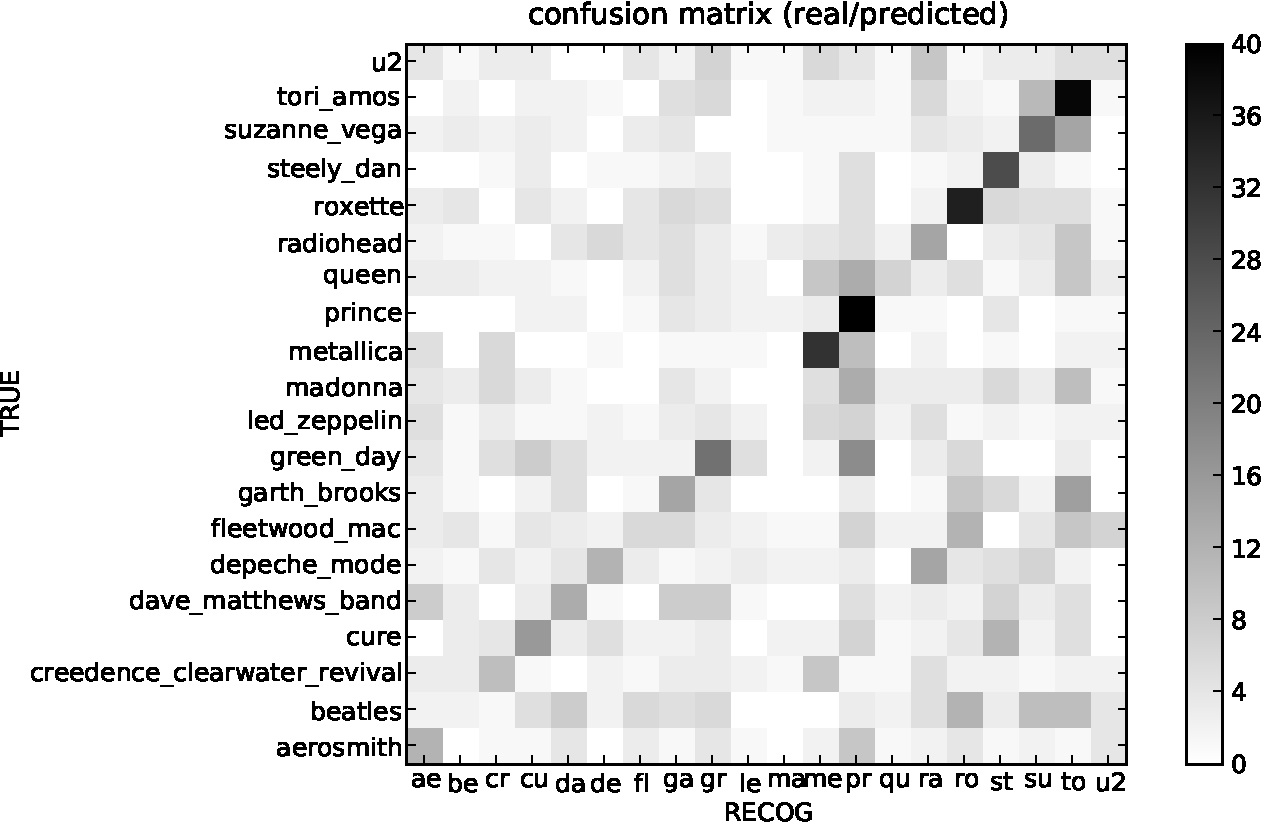
\includegraphics[width=0.48\textwidth]{conf_mat_per_artist.ps}
  \end{center}
  \vspace{-20pt}
\end{wrapfigure}

\textbf{Artist recognition task}.
We use the {\it artist20} data set: $1402$ songs from $20$ artists, 
mostly rock and pop of different subgenres.  
Previously published results using GMMs on MFCC features achieve an 
accuracy of $59\%$, whereas using only chroma as a representation yields an
accuracy of $33\%$  \cite{Ellis2007}.

We get an accuracy of $\mathbf{23.4\%}$, random baseline 
is around $5\%$. 
The confusion matrix is shown here, note 
that certain artists are recognized at an accuracy far above the average.

\end{minipage}

\vspace{2cm}

\begin{minipage}[c][9cm][c]{\columnwidth}
  %\begin{center}
\textbf{Bar alignment task}.
Since the clustering described is based
on the segmentation of the signal in to bars, 
the codewords should contain information related to bar
alignment, such as the presence of a strong beat on the first beat.\\
  %\end{center}
\end{minipage}
\begin{minipage}[c][9cm][c]{0.21\textwidth}
  \begin{center}
      \begin{tabular}{cc}
        Offset & \% of times chosen \\ \hline \hline
        0 & $\mathbf{62.6}$\\
        1 & $16.5$\\
        2 & $9.4$\\
        3 & $11.5$
      \end{tabular}
      %\mytablecaption{\small{
      %    Bar alignment experiment:
      %    offsets relative to ground-truth 4-beat bar boundaries 
      %    that gave minimum distortion encodings from the bar-aligned codebook.
      %}}
      \label{tab:offset}
  \end{center}
\end{minipage}

\begin{list}{\labelitemi}{\leftmargin=2em \labelsep=1em}
\item A bullet point
\item A bullet point
\item A bullet point
\item A bullet point
\end{list}


%%% Section 6
\vspace{0cm}
\begin{center}
  \pbox{0.8\columnwidth}{}{linewidth=2mm,framearc=0.1,linecolor=lightred,fillstyle=gradient,gradangle=0,gradbegin=white,gradend=whitepink,gradmidpoint=1.0,framesep=1em}{
    \begin{center}
      \large Conclusion
    \end{center}}
\end{center}

\vspace{1.0cm}

\begin{list}{\labelitemi}{\leftmargin=2em \labelsep=1em}
\item A bullet point
\item A bullet point
\end{list}




%%% References
\begin{small}
\bibliographystyle{IEEEtran}
\bibliography{tbm_bib}
\end{small}

\end{multicols}

% FOOTNOTE
\vspace{1cm}
\begin{minipage}{\textwidth}
\begin{small}
\begin{flushright}
Poster presented at ISMIR 2010 (Utrecht) for the paper:
Clustering Beat-Chroma Patterns in a Large Music Database by
T. Bertin-Mahieux, R. J. Weiss and D. P. W. Ellis. Contact:
\url{tb2332@columbia.edu}, code: \url{http://www.columbia.edu/~tb2332/}.
\end{flushright}
\end{small}
\end{minipage}

\end{poster}
\end{document}

